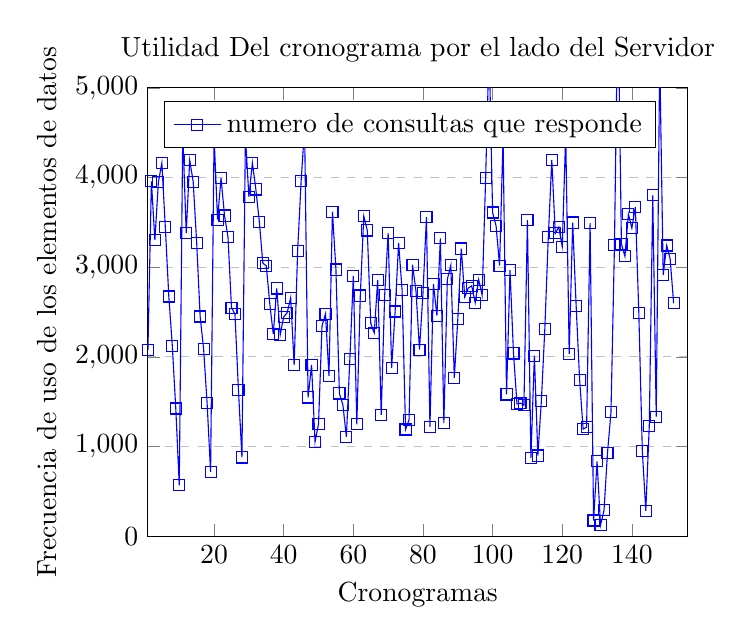
\begin{tikzpicture}
\begin{axis}[
    title={Utilidad Del cronograma por el lado del Servidor},
    xlabel={Cronogramas},
    ylabel={Frecuencia de uso de los elementos de datos},
    xmin=1, xmax=156,
    ymin=0, ymax=5000,
    xtick={},
    ytick={},
    legend pos=north west,
    ymajorgrids=true,
    grid style=dashed,
]

\addplot[
    color=blue,
    mark=square,
    ]
    coordinates {
%UTILIDAD TOTAL
(1,2076)
(2,3958)
(3,3301)
(4,3948)
(5,4161)
(6,3444)
(7,2673)
(8,2124)
(9,1424)
(10,567)
(11,4499)
(12,3379)
(13,4194)
(14,3954)
(15,3274)
(16,2450)
(17,2085)
(18,1482)
(19,716)
(20,4462)
(21,3530)
(22,3995)
(23,3576)
(24,3334)
(25,2549)
(26,2476)
(27,1630)
(28,878)
(29,4462)
(30,3785)
(31,4163)
(32,3867)
(33,3506)
(34,3046)
(35,3015)
(36,2593)
(37,2253)
(38,2763)
(39,2248)
(40,2446)
(41,2493)
(42,2661)
(43,1909)
(44,3185)
(45,3957)
(46,4560)
(47,1547)
(48,1909)
(49,1053)
(50,1251)
(51,2345)
(52,2481)
(53,1788)
(54,3619)
(55,2974)
(56,1592)
(57,1465)
(58,1107)
(59,1978)
(60,2902)
(61,1248)
(62,2684)
(63,3570)
(64,3410)
(65,2374)
(66,2267)
(67,2859)
(68,1353)
(69,2690)
(70,3379)
(71,1876)
(72,2506)
(73,3270)
(74,2746)
(75,1190)
(76,1297)
(77,3027)
(78,2731)
(79,2081)
(80,2711)
(81,3558)
(82,1220)
(83,2813)
(84,2460)
(85,3322)
(86,1261)
(87,2865)
(88,3020)
(89,1767)
(90,2418)
(91,3208)
(92,2667)
(93,2767)
(94,2792)
(95,2605)
(96,2861)
(97,2687)
(98,3994)
(99,5471)
(100,3610)
(101,3461)
(102,3017)
(103,4442)
(104,1581)
(105,2967)
(106,2038)
(107,1475)
(108,1484)
(109,1460)
(110,3524)
(111,871)
(112,2014)
(113,899)
(114,1505)
(115,2313)
(116,3337)
(117,4194)
(118,3377)
(119,3448)
(120,3229)
(121,4479)
(122,2034)
(123,3498)
(124,2565)
(125,1740)
(126,1194)
(127,1215)
(128,3492)
(129,175)
(130,834)
(131,124)
(132,288)
(133,930)
(134,1382)
(135,3245)
(136,6069)
(137,3261)
(138,3122)
(139,3591)
(140,3436)
(141,3670)
(142,2486)
(143,954)
(144,283)
(145,1230)
(146,3802)
(147,1333)
(148,5348)
(149,2915)
(150,3242)
(151,3091)
(152,2597)
    };
    \legend{numero de consultas que responde}

\end{axis}
\end{tikzpicture}

